\documentclass{VUMIFPSkursinis}
\usepackage{algorithmicx}
\usepackage{algorithm}
\usepackage{algpseudocode}
\usepackage{amsfonts}
\usepackage{amsmath}
\usepackage{array}
\usepackage{bm}
\usepackage{caption}
\usepackage{color}
\usepackage{float}
\usepackage{graphicx}
\usepackage{listings}
\usepackage{longtable}
\usepackage{subfig}
\usepackage{wrapfig}
\usepackage{enumitem}

\usepackage[tableposition=top]{caption}
%PAKEISTA, tarpai tarp sąrašo elementų
\setitemize{noitemsep,topsep=0pt,parsep=0pt,partopsep=0pt}
\setenumerate{noitemsep,topsep=0pt,parsep=0pt,partopsep=0pt}

\newcolumntype{L}[1]{>{\raggedright\let\newline\\\arraybackslash\hspace{0pt}}m{#1}}
\newcolumntype{C}[1]{>{\centering\let\newline\\\arraybackslash\hspace{0pt}}m{#1}}
\newcolumntype{R}[1]{>{\raggedleft\let\newline\\\arraybackslash\hspace{0pt}}m{#1}}

% Titulinio aprašas
\university{Vilniaus universitetas}
\faculty{Matematikos ir informatikos fakultetas}
\department{Programų sistemų katedra}
\papertype{Individualus PKP temos nagrinėjimas}
\title{Literatūros šaltinio analizė}
\titleineng{Initiating software process improvement in very small enterprises
Experience with a light assessment tool}
\status{4 kurso 3 grupės studentas}
\author{Gediminas Krasauskas}
\supervisor{prof. dr. Andrius Adamonis}
\date{Vilnius – \the\year}

% Nustatymai
% \setmainfont{Palemonas}   % Pakeisti teksto šriftą į Palemonas (turi būti įdiegtas sistemoje)
\bibliography{bibliografija}

\begin{document}
\maketitle

\tableofcontents

\sectionnonum{Įvadas}
Ši literatūros šaltinio analizė apima glaustą pagrindinių literatūros šaltinio \cite{habra2008initiating} idėjų ir išvadų išdėstymą bei tų idėjų ir išvadų kritinę analizę – pateikiant argumentus tiek patvirtinančius išsakytas idėjas, tiek prieštaraujančius joms. 

Mokslinis straipsnis buvo parašytas 2006 metais, publikuotas 2008 metais, o prie jo prisidėjo 5 autoriai. Tačiau jo tematikos aktualumas dėl jos universalumo nėra mažesnis praėjus ir kiek daugiau nei 10 metų.

Pagrindinio mokslinio šaltinio esmė yra programinės įrangos procesų tobulinimas labai mažose įmonėse (angl. \textit{Very Small Enterprises}), naudojant lengvą ir tam pritaikytą įrankį, sudarytą iš 3 žingsnių, iš kurių ties vienu yra koncentruojamasi labiausiai.

Tyrimą galima laikyti pagrįstu, kadangi aprašytos praktikos, anot autorių, buvo naudotos net septynerius metus 86 įmonėse, esančiose 3 skirtingose šalyse.

Teksto apimtis - 1396 žodžiai.

\section{Analizė}
Peršasi mintis, kad autorių motyvaciją tyrimui kyla iš problemos, kad didelės įmonės, žinodamos programų kūrimo procesų (toliau PKP) gerinimo svarbą, naudoja standartizuotus PKP kokybės gerinimo įrankius arba susikuria juos pagal savo poreikius. Tačiau labai mažos įmonės (toliau LMĮ) tam paprasčiausiai neskiria resursų, nes neturi išgalių, t.y. tokia veikla reikalauja didelių investicijų ir yra labai sudėtinga. Iš tiesų, daug tyrimų patvirtina, kad procesų gerinimas reikalauja didelio kapitalo \cite{humphrey1991software} \cite{herbsleb1994benefits} \cite{diaz1997software} \cite{van2004measuring}, kurio mažos įmonės paprasčiausiai neturi. 

Šioje vietoje autoriai teisingai pastebi, kad tai lemia žemą LMĮ PKP brandos lygį dėl mažo arba beveik visai neskiriamo dėmesio procesų kokybės užtikrinimui ir jų gerinimui. Ko gero tai lemia, kad LMĮ nukenčia bendrieji procesai, tokie kaip kokybės užtikrinimas, reikalavimų analizė ir t.t., kurie yra svarbūs tokiuose brandos lygio vertinimo modeliuose, kaip CMMI \cite{peldzius2011comparison}. Tačiau, nepaisant to, LMĮ dažnai turi puikiai atliekamas smulkias specifines technines veiklas. Tai reiškia, kad skyrus santykinai nedaug resursų disciplinuotai ir tikslingai pagerinti PKP, galima pasiekti teigiamų pokyčių LMĮ procesuose. Tuo ir remiasi autorių pristatomas OWPL palaipsniškas PKP gerinimo būdas.

\subsection{LMĮ analizė}
Autoriai, remdamiesi savo patirtimi ir stebėjimais, išskiria procesų charakteristikas, būdingas LMĮ. 
\begin{itemize}
    \item PĮ gyvavimo ciklas supaprastintas, pagrindinės fazės nėra formalizuotos, o vienas iš svarbiausių etapų - testavimas - yra praleidžiamas pro pirštus, kad būtų telpama į laiko ir biudžeto rėmus. Toks požiūris, taupant testavimo sąskaita, gali atrodyti pragmatiškas, tačiau dažnai veda į projekto nesėkmę \cite{charette2005software}.
    \item Procesų brandos lygiai toje pačioje organizacijoje gali labai skirtis. Iš dalies galima sutikti, kad mažose įmonėse tai yra vyraujanti tendencija, tačiau didelės įmonės ko gero taip pat susiduria su šia problema. Ypač, jeigu jos nesiekia laimėti konkursų projektams, kuriuose tam tikri brandos lygiai pagal standartus yra privalomi.
    \item Kokybės užtikrinimo ir rizikų valdymo stoka. Tą ko gero lemia LMĮ \textit{ad-hoc} praktika, kuri techniškai kainuoja ženkliai mažiau. Tačiau tikėtina, kad PKP gerinimo motyvaciją tiesiogiai įtakoja požiūris, atsirandantis visoje organizacijoje dėl kokybės užtikrinimui mažai skiriamo dėmesio. Tiesa, rizikų valdymo stoka gali sukurti aukštos rizikos - didelio atlygio efektą, kuomet startuoliai prisiėmę labai aukštą riziką gali patirti milžinišką sėkmę.
    \item LMĮ neskiria arba skiria labai mažai dėmesio darbuotojų apmokymui. Tai atrodo logiška, nes tokie mokymai kainuoja didelius pinigus ir įmonė galbūt tikisi, kad darbuotojas savarankiškai išmoks dalykus, reikalingus sklandžiai vykdyti darbus. Tačiau tai vis tiek potencialiai sukelia aukštą riziką, kad darbas sustos, nes dalis darbuotojų paprasčiausiai neturės kompetencijų vykdyti užduotis, reikalaujančias specifinių aukšto lygio žinių.
    \item Didžiojoje dalyje LMĮ neaptinkama procesų, liečiančių projektų planavimo ir valdymo praktikas. Tikėtina, kad šį reiškinį eilinį kartą lemia resursų stoka, tačiau daugelis sutinka, jog projektų rezultatai dažnai koreliuoja su puikiais projekto vadovo įgūdžiais - Tarptautinė projektų valdymo asociacija (IPMA) nustatė, kad geras projektų valdymas leidžia sutrumpinti projektų atlikimo trukmę vidutiniškai 20–30\%, o išlaidas sumažinti 10–15\%. Vis dėlto galima teigti, kad didesnius projektus dėl apimties yra sunkiau suplanuoti ir valdyti, nei mažesnius, todėl ten šie procesai yra labiau reikalingi.
    \item ISO organizacija yra pareiškusi, kad tarptautiniai PĮ standartai yra sunkiai pritaikomi LMĮ.
\end{itemize}

\subsection{OWPL metodas}
Autoriai aprašo OWPL metodą, paremtą palaipsnišku 3 fazių PKP gerinimo vertinimu, sudarytu iš: mikrovertinimo, OWPL vertinimo ir SPICE arba CMM/CMMi vertinimo. Kiekvienos žemiau esančios fazės vertinimo duomenys naudojami aukštesnio lygio vertinime, kur aukštesnio lygio vertinimą galima atlikti su vis didesniu tikslumu. Toks įrankis yra patogus ne tik mažoms įmonėms, bet ir vidutinio dydžio organizacijoms. Įrankis suteikia lankstumo, t.y. įmonė nebūtinai turi atlikti visus žingsnius ir gali sustoti tame etape, kuriame jaučia, jog gavo pakankamai duomenų gerinti vidinius procesus. Tiesa, tai ko gero būtų nelabai tinkamas variantas didelėms įmonėms, nes įrankis vis dėlto nesuteikia tokių tikslių duomenų, kurių galbūt būtų tikimasi, lyginant su kitais įrankiais.

\subsection{Mikrovertinimo modelis ir įrankis}
Toliau straipsnyje visas dėmesys skiriamas vienam iš OWPL fazių - mikrovertinimui, t.y. jo modeliui ir įrankiui. Kaip autoriai tikina, konferencijos, diskusijos, išreikštinis mažų organizacijų poreikis rodė, kad egzistuoja rimtas susirūpinimas, liečiantis PĮ kokybės klausimą. Šitaip atsirado mikrovertinimo įrankio pradinė versija, kurios naudą reikėjo išbandyti praktikoje. Įrankį išbandė 20 organizacijų, iš kurių visos buvo patenkintos rezultatais ir suteikė grįžtamą ryšį, kuris buvo panaudotas įrankio tobulinimui, o vėliau atsirado ir daugiau partnerių kitose šalyse.

Mikrovertinimu autoriai siekia suteikti pradinį PĮ praktikų vertinimą už kuo mažesnę kainą, t.y. LMĮ supažindinti su jos stiprybėmis ir silpnybėmis, potencialiais pagerinimais ir tuos pagerinimus suskirstyti pagal svarbą. Tačiau strateginis įrankio tikslas - pagerinti bendrą PĮ praktikų brandos lygį. Kyla abejonių, ar šis tikslas nėra antrinis. Didesnėms įmonėms tam tikrais atvejais yra naudingas tikslas formaliai pasiekti aukštesnį praktikų brandos lygį, kad būtų galima dalyvauti ir laimėti konkursus. Tačiau mažoms įmonėms žymiai naudingiau yra gauti praktinę naudą, t.y. pradėti vykdyti procesus ir naudoti praktikas, kurių anksčiau nenaudojo ir apie kurias nežinojo, atsirinkti bei gerinti svarbiausius procesus, atnešančius įmonei didžiausią pridėtinę vertę.

Procese yra naudojamas klausimynas, kurį interviu metu naudoja vertintojas ir įmonės įgaliotas asmuo. Anot autorių, vertintojas privalo turėti žinių PĮ kokybės, procesų gerinimų ir organizacijos IT veiklų srityse. Tai esą leidžia interviu padaryti našesnį ir išvengti nesuprastų klausimų. Tai yra įvardijama labiau kaip informacijos apsikeitimas nei auditas. Šios taisyklės leidžia suprasti, kad įmonei būtų patogu, jei tokį vertinimą atliktų darbuotojas iš pačios organizacijos, nes jis turėtų daug žinių apie organizaciją ir joje vykstančius procesus, papildomai prieš tai apmokius jį PĮ kokybės ir proceso gerinimo srityse. Tačiau tai gali sukelti riziką, nes darbuotojui būtų sunku iki galo išlikti objektyviam. Kitas variantas būtų samdyti išorinį vertintoją, pavyzdžiui konsultantą. Tačiau tai lemtų didesnius kaštus - užtruktų vertintojo supažindinimas su organizacijos IT srities veiklomis. Šaltinio autoriai nepateikia tinkamos strategijos arba minčių šiuo klausimu.

Siekiant nuoseklios mažų kaštų strategijos, autoriai nurodo interviu formatą, kurio trukmė nuo 45 iki 60 minučių su galimų telefoninių skambučių alternatyva. Patį klausimyną sudaro 18 užklausų, iš kurių absoliuti dauguma skirta 6 pagrindinėms praktikų sritims: kokybės valdymui, klientų valdymui, subrangovų valdymui, projekto kūrimui ir valdymui, produkto valdymui ir mokymų bei žmogiškųjų išteklių valdymui. Kiekvienos užklausos struktūra - klausimas ir tada vienas arba daugiau sekančių papildančių klausimų. 

Gauti atsakymai leidžia sumodeliuoti brandos profilio diagramas, kurias nesudėtinga lyginti tarpusavyje matuojant progresą (žr. Priedas nr. 1). Tačiau toks modelis yra patogus tik labai apibendrintam paveikslui susidaryti. Net jei ir matytume užklausų ir atsakymų išklotinę, toks ribotas klausimo-atsakymo informacijos rinkimo metodas negali atskleisti detalių apie konkrečius procesus, dėl to sunku daryti gilumines išvadas apie įmonės naudojamas praktikas. Šis būdas gali pateikti atsakymus į klausimą \textit{kas}, tačiau ne į klausimą \textit{kaip}. Autoriai taip pat nepateikia paaiškinimo, kodėl pasirinktos būtent šios šešios sritys.

Mikrovertinimo ataskaitą parengia vertintojai. Joje įmonė gali matyti apibendrintus rezultatus, pateiktus remiantis įmonės 6 procesų ašimis. Rezultatai turi būti pateikti įmonės kontekste, kad būtų kuo daugiau naudos. Tada stiprybės, silpnybės, rekomendacijos ir gerinimo veiklos, išdėstytos prioriteto tvarka. Šioje vietoje autoriai pabrėžia, kad LMĮ, kuri pasiekia aukštesnį lygį, toliau turėtų pereiti į kitą įrankio pakopą ir naudoti pažangesnį, OWPL metodą.

\subsection{Rezultatai}
Autoriai detaliai nagrinėja rezultatus pasitelkdami geografinį aspektą, t.y. apibendrina kiekvienoje geografinėje vietoje atliktus stebėjimus: Valonijoje, Kvebeke ir Prancūzijoje, išskirdami kaip organizacijoms sekėsi pasiekti apibrėžtus lygius. Kyla klausimas, ką tiksliai atskleidžia geografinis aspektas, nes rezultatai gali skirtis dėl kultūrinių šalių skirtumų, o tai nėra labai naudingi duomenys norint prieiti prie išvadų procesų brandos kontekste. Buvo bandoma nupiešti globalų vaizdą, tačiau čia galima sutikti su autoriais, jog pastaroji diagrama nesuteikia naudingos informacijos - rezultatai nežymiai skiriasi. Autoriai pabrėžia, kad tyrime nėra kreipiama dėmesio į tokius parametrus, kaip projekto tipas, dydis, rinka ir t.t. Galbūt tai yra viena iš tyrimo silpnybių. Įtraukus į tyrimą, pavyzdžiui, projekto dydžio arba tipo atributus galėtume sužinoti, kokiose rinkose kokie procesai LMĮ yra linkę būti aukštesnio lygio ir panašiai. Manipuliuodami šiais duomenimis tikėtina, kad aptiktume ir daugiau tendencijų. Vis dėlto reikėtų suprasti autorius - negalime atmesti kompleksiškumo faktoriaus, dėl kurio įtraukiant vis daugiau parametrų, tyrimą būtų gerokai sudėtingiau atlikti.

Toliau autoriai apibendrino ir pateikė trumpų įžvalgų apie kiekvieną iš 6 procesų ašių. Vienas iš esminių momentų, kuriuos pastebėjo autoriai yra tas, kad projektų gyvavimo ciklas ir sukuriamų produktų struktūra pasirodė gana gerai, bet praktikos, liečiančios PĮ kūrimo metodologiją pasiekė mažą įvertinimą. Tai buvo argumentuojama tuo, kad nors mažos įmonės ir kuria bei naudoja dokumentų standartizuotus ir atsekamus šablonus, tačiau to oficialiai neapibrėžia. Net jeigu organizacijoje šios praktikos veikia, deja nėra tai patvirtinančių formalių įrodymų.

\subsection{Išvados}
Išvadose autoriai išskiria teigiamas mikrovertinimo savybes: supaprastintas mažų kaštų vertinimo būdas, tikslus įrankis norint pradėti organizcijos vertinimą, palaipsniškas būdas su pakopiniais vertinimo ciklais, į kontekstą atsižvelgiantis būdas, supaprastintas žodynas.

Išskiriamos ir neigiamos mikrovertinimo savybės: interviu metu sukauptos žinios nėra laikytinos vienareikšmiškai patikimos, įrankis neatsižvelgia į nedisciplinuotas kūrimo praktikas, pavyzdžiui \textit{agile}, praktikoje įrankis buvo pritaikytas tik vienam įmonės projektui ar komandai, todėl kitiems projektams ar komandoms efektyvumas nebuvo pamatuotas.

\sectionnonum{Santrumpos ir apibrėžimai}

\textbf{LMĮ} – labai maža įmonė.

\textbf{PKP} – Programų kūrimo procesas.

\textbf{PĮ} – Programinė įranga.

\textbf{CMMI} – Capability Maturity Model Integration.

\textbf{OWPL} – Observatoire Wallon des Pratiques Logicielles.

\textbf{SPICE} – Software Process Improvement and Capability Determination.

\textbf{Agile} – Lanksčiojo programavimo programų kūrimo metodologija.

\printbibliography[heading=bibintoc]

\clearpage

\appendix 

\section{Standartinis verslo tinklo modelis}
\begin{figure}[H]
    \centering
    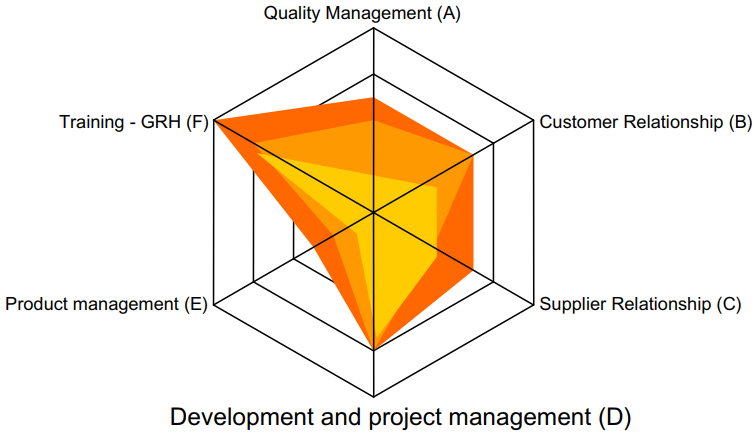
\includegraphics[scale=0.75]{img/diagrama.PNG}
    \caption{Brandos profilio diagrama}
    \label{img:pav-1}
\end{figure}

\end{document}
